% Appendix1 file from standard thesis template
\appendixtitle
\appendix
\chapter{SOURCE CODE} \label{appendix1}
This appendix contains a copy of the source code used to create a total power radiometer in software and software that is able to load and parse information stored from this SDR-based radiometer.  The first code displayed is the source code that creates the total power radiometer in software and analyzes the data generated from the SDR-based radiometer. The first code is the heir block created that detects the power and smooths the data.  An heir block is a user created block that is used in GNURadio Companion.  The second code supplied is Python code that could be used to read the data generated from the SDR-based radiometer and plot it.  This provides an example of reading and parsing data generated from our SDR-based radiometer.

The code included in this appendix is provided as a point of reference.  It may be out of date or incomplete.  Copies of this thesis' source \LaTeX code, most experimental data, and additional code used may be found on the author's GitHub repository, \url{https://github.com/matgyver/Radiometer-SDR-Thesis}.

\section*{Python code for total power radiometer}
This code defines a custom block in GNURadio Companion (GRC) that detects power, smooths the data and then decimates the data to reduce the storage size. This heir block may then be imported in GNURadio Companion and used like any other block in GRC.  A screenshot of this block is shown in Figure \ref{TPR_GRC}.

{\begin{figure}[h!tb] 
\centering
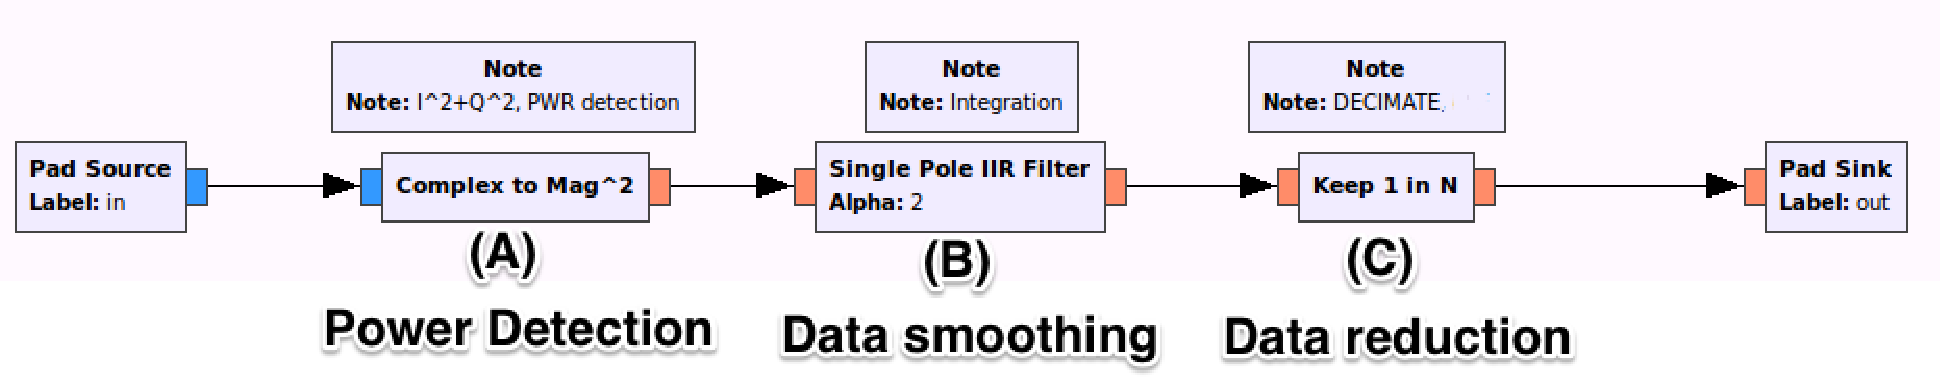
\includegraphics[width=0.8\linewidth]{Images/TPR_grc.png}
\isucaption{Blocks used for creating a total power radiometer in software.  Source: GNURadio Companion}
\label{TPR_GRC}
\end{figure}
}


\lstset{
  language=Python,
  showstringspaces=false,
  formfeed=\newpage,
  tabsize=4,
  commentstyle=\itshape,
  basicstyle=\ttfamily,
  breaklines=true,
  morekeywords={models, lambda, forms}
}

\newcommand{\code}[2]{
  \hrulefill
  \subsection*{#1}
  \lstinputlisting{#2}
  \vspace{2em}
}

\code{Total Power Radiometer Block}{Code/TPR.py}
\newpage

%\section*{Matlab code for reading and displaying data from GNURadio}
%\lstset{
%  language=Matlab,
%  showstringspaces=false,
%  formfeed=\newpage,
%  tabsize=4,
%  commentstyle=\itshape,
%  basicstyle=\ttfamily,
%  morekeywords={models, lambda, forms}
%}

%\newcommand{\matlabcode}[2]{
%  \hrulefill
%  \subsection*{#1}
%  \lstinputlisting{#2}
%  \vspace{2em}
%}

%\matlabcode{GNURadio Parsing Code}{Code/gnuradio_parse.m}
%\newpage

\section*{Python code for analyzing data}
IPython notebooks was used to perform an analysis on the data used in this thesis.  The code presented here is an example of using iPython to read and parse data from the SDR-based radiometer.  The Markdown language as well as some HTML is used to create easy to read pages that include the python code, generated graphs and descriptive text.  
\lstset{
  language=Python,
  showstringspaces=false,
  formfeed=\newpage,
  tabsize=4,
  commentstyle=\itshape,
  basicstyle=\ttfamily,
  morekeywords={models, lambda, forms}
}

\newcommand{\pythoncode}[2]{
  \hrulefill
  \subsection*{#1}
  \lstinputlisting{#2}
  \vspace{2em}
}

\pythoncode{Total Power Radiometer}{Code/iPython/Radiometer_Parse.py}
%\newpage